\section{Rendering 3D}
\label{sec:chapter_stato_arte_rendering3d}

Per Rendering si intende il processo di generazione di un’ immagine a due dimensioni a partire una scena a tre dimensioni.
Ogni scena rappresenta un  ambiente contenente principalmente oggetti, luci e camere.
Gli oggetti sono entità 3D composte da una geometria ed un materiale che rispettivamente ne definiscono forma ed aspetto. Queste entità possono essere soggette a trasformazioni che ne alterano posizione, rotazione e scalatura all’interno dello spazio tridimensionale della scena.
La visibilità di un oggetto può essere alterata dalla presenza o meno di sorgenti luminose, così come dalla presenza di camere.
Ogni camera definisce un volume di vista all’ interno della scena; solamente gli oggetti contenuti in questo volume sono renderizzati.
\\
\begin{figure}[htb]
 \centering
 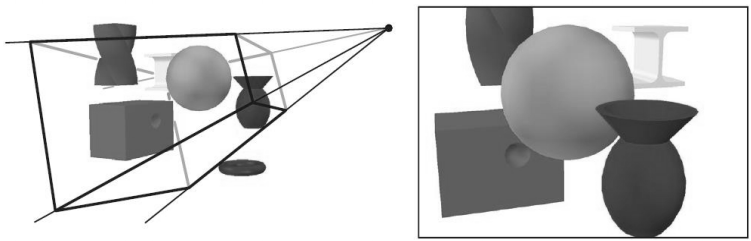
\includegraphics[width=0.9\linewidth]{images/chapter_stato_arte/stato_arte_rendering_3d.png}\hfill
 \caption[Rendering 3D]{A sinistra una scena 3D, a destra un render 2D}
 \label{fig:stato_arte_rendering_3d}
\end{figure}
\\
In un ambiente grafico 3D è possibile pre-rendirizzare una scena (pre-rendering) o renderizzarla in tempo reale (real-time rendering).
\\
Il rendering real time permette la generazione di un flusso di immagini intervallate da brevi istanti di tempo.
È un processo interattivo in quanto ogni immagine da esso generata rappresenta il feedback dell’interazione dell’osservatore con l’immagine precedente.
\\ 
Si viene a creare un ciclo che prevede il rendering e l’interazione con l’immagine renderizzata, e ciò avviene con una velocità tale per cui l’osservatore non vede le singole immagini, ma un unico processo dinamico.
\\ 
La rapidità con cui le immagini vengono mostrate su schermo è misurata in frame per secondo (FPS): maggiore è l’FPS, minore è il tempo di risposta ad un azione dell’osservatore, migliore è l’interattività.
\\ 
Allo stato attuale, il rendering in real-time è possibile grazie all’esistenza di componenti hardware dedicate all’accelerazione grafica: le unità di processamento grafico, o GPU. 
Esse sono in grado di gestire, ad ogni frame, milioni se non miliardi di pixel. 
\\
Tuttavia è importante sottolineare il fatto che il rendering real-time produce risultati qualitativamente peggiori rispetto ad un rendering off-line (o pre-rendering), anche se il divario tra i due tende ad assottigliarsi. 
\\

Il pre-rendering è il processo nel quale le immagini da mostrare non vengono renderizzate in tempo reale dall’ hardware che lo effettua. Piuttosto esse vengono renderizzate precedentemente da un hardware differente, tipicamente più potente di quello utilizzato, e poi proiettate su schermo.
\\
Il processo di fatto permette di diminuire enormemente il carico di lavoro della macchina addetta alla riproduzione video, in quanto essa si limita solamente a mostrare immagini pre-calcolate da un’ altra macchina senza effettuare alcun calcolo di rendering.
\\
Ne consegue un processo computazionalmente oneroso per l’ hardware che lo effettua ma molto efficiente per la macchina che riproduce il video, permettendole di utilizzare modelli grafici più complessi di quelli che sarebbe riuscita a renderizzare in real-time.
\\
I primi impieghi di questa tecnica risalgono all’ inizio degli anni 90 per permettere realizzazioni grafiche ad altissimo livello di realismo, nettamente superiore a quella ottenibile in real-time, e viene utilizzata ancora oggi principalmente per la creazione di film o videogiochi.
Nel 1991 nacquero i primi videogiochi che ne facevano uso, e già nel 1995 venne creato il primo film 3D completamente prerenderizzato: Toy Story.
In quegli anni la grafica pre-renderizzata nei giochi era utilizzata principalmente per la realizzazione di cut-scene fotorealistiche e sfondi prerenderizzati.
\\
Videogiochi come Resident Evil e Final Fantasy sulla prima Playstation fecero largo uso di questa tecnica e contribuirono a renderla famosa fino all’inizio degli anni 2000. 
Verso la fine degli anni 90 questa tecnica ha permesso di ottenere enormi miglioramenti grafici; la figura mette in comparazione un’ immagine che fa utilizzo di sfondi prerenderizzati con una renderizzata in tempo reale.
\\
\begin{figure}[htb]
 \centering
 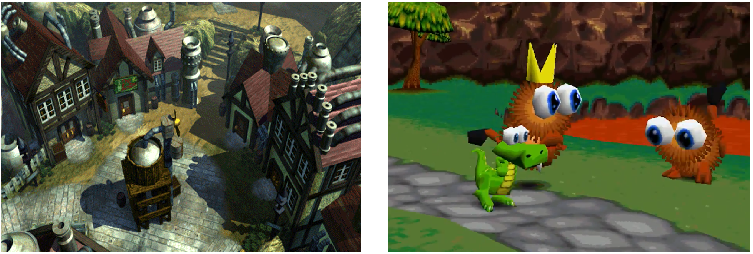
\includegraphics[width=1\linewidth]{images/chapter_stato_arte/stato_arte_croc_ffvii.png}\hfill
 \caption[Confronto tra scena prerenderizzata e real time]{A sinistra una scena prerenderizzata (Final Fantasy VII, 1997), a destra una scena renderizzata in tempo reale (Croc, 1997)}
 \label{fig:stato_arte_confronto_ffvii_croc}
\end{figure}
\\
Lo svantaggio derivante dall’utilizzo di sfondi prerenderizzati risiede però nel basso livello di interattività del personaggio giocante con la scena.
\\
Lo sfondo (o scena) infatti rimane fisso, in quanto l’hardware su cui viene eseguito il gioco non effettuare calcoli real-time ma mostra solamente l’immagine di rendering ottenuta da un hardware molto più potente.
\\
Questo comporta l’impossibilità di muovere la telecamera a proprio piacimento all’interno della scena, cosa possibile invece con il rendering real-time. La camera risulta infatti immobile e permette solamente di osservare la scena dal medesimo punto di osservazione con cui è stata renderizzata dall’hardware più potente. Di fatto è come se l’hardware meno potente mostrasse una fotografia scattata dall’hardware più potente.
\\
Il prerendering inoltre rende impossibile modificare le ombre e le luci dello sfondo in quanto anch’esse rimangono fisse; solamente un approccio real-time permette di calcolarle e quindi modificarle dinamicamente.
\\
Con l’aumentare della potenza degli hardware disponibili sul mercato però già dopo i primi anni 2000 l’utilizzo degli sfondi prerenderizzati è iniziato a diminuire. Le nuove macchine hanno permesso infatti la creazione di convincenti scene 3D in real-time.
\\ 
Nei giorni d’oggi la maggior parte dei giochi sono quasi interamente realizzati tramite rendering real-time. A differenza però degli sfondi prerenderizzati che sono stati completamente abbandonati, i filmati prerenderizzati vengono ancora ampiamente creati, nonostante la differenza con quelli real-time si sia molto assottigliata (\ref{fig:stato_arte_cutscenes}).
\\
\begin{figure}[htb]
 \centering
 
\includegraphics[width=1\linewidth]{images/chapter_stato_arte/stato_arte_tw.png}\hfill
 \caption[Confronto tra cutscene moderne prerenderizzate e real time]{A sinistra una cutscene prerenderizzata, a destra una cutscene renderizzata in tempo reale (The Witcher 3,  2015)}
 \label{fig:stato_arte_cutscenes}
\end{figure}
\\
Attualmente, nonostante la grafica sia quasi completamente real-time, vengono utilizzati differenti metodi di pre-rendering  che alleggeriscono il carico di lavoro del rendering real-time. Metodi quali ad esempio le lightmap che permettono l’utilizzo di luci ed ombre precalcolate, non richiedendo di doverle calcolare real-time, o le env-map precomputate che permettono di alleggerire il carico di lavoro dovuto al calcolo di superfici riflettenti o rifrangenti.
\\
Proprio queste due tecniche, che saranno analizzate nel dettaglio successivamente, vengono utilizzate in questo lavoro di tirocinio per permettere la fruizione di ambienti fotorealistici anche su hardware con prestazioni non elevate. 
\\
Nel presente lavoro di tesi viene utilizzato un approccio misto di prerenderizzazione unito ad una renderizzazione real-time.
Il rendering real-time risulta necessario per permettere il movimento della camera all’interno della scena, inoltre la precomputazione permette il calcolo offline delle informazioni di luce tramite l’utilizzo di un hardware estremamente performante.